\chapter{Introduction}

\section{Background}

\section{Previous work}

\section{Research goals}

\begin{figure*}
    \centering
    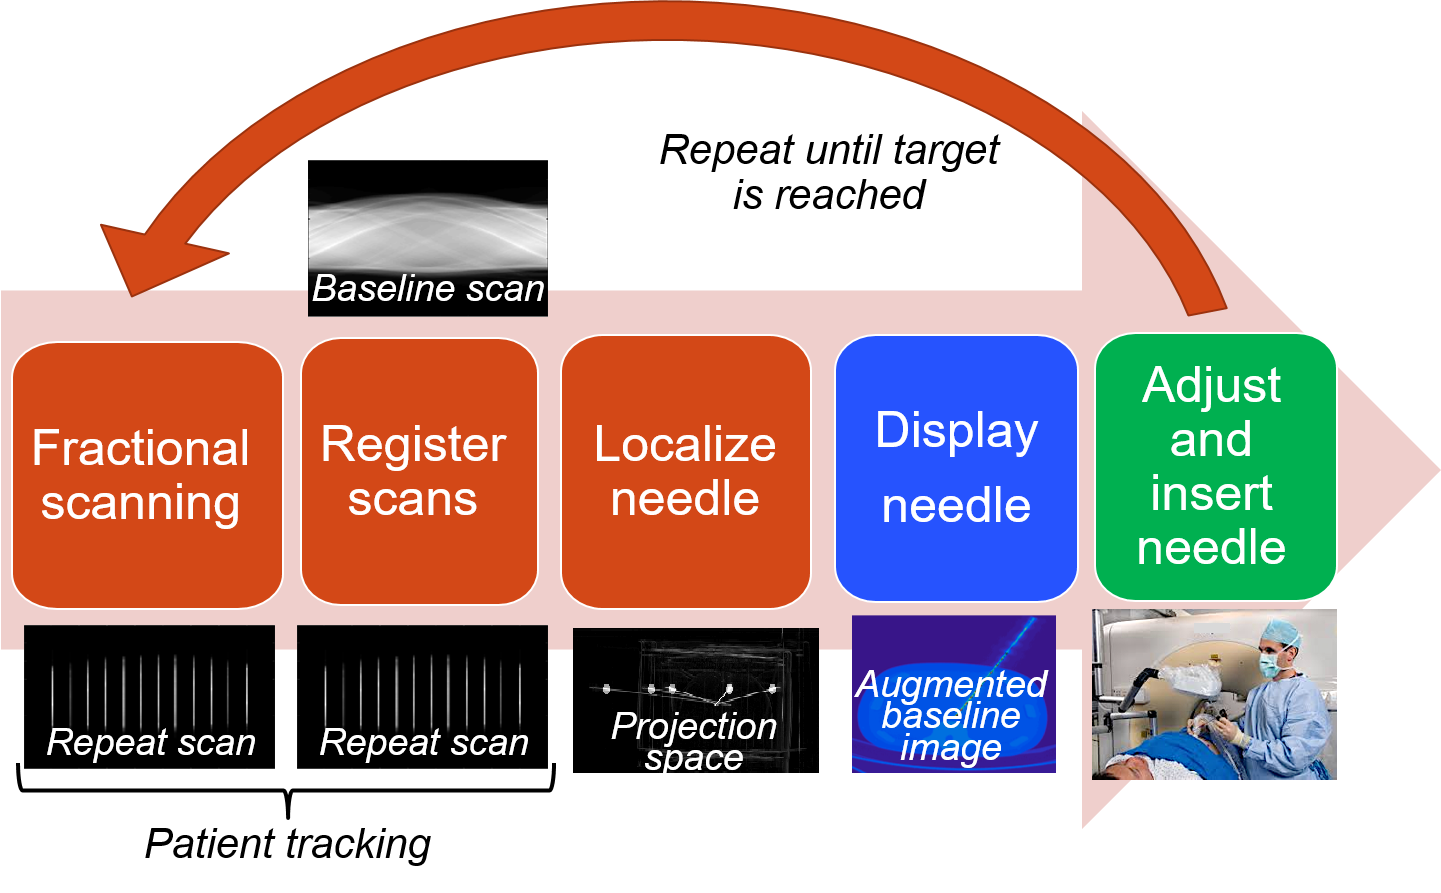
\includegraphics[width=\textwidth]{figures/needle+patient_tracking.png}
    \caption{Illustration of image-less needle and patient tracking process in interventional radiology.
}
    \label{fig:figures/needle+patient_tracking.png}
\end{figure*}

\textbf{The first goal of this thesis is to develop and validate an algorithm for rigid registration in repeat CT scanning procedures based on Radon-space methods achieving an x-ray dose reduction.}

The focus of this thesis is to develop methods taking advantage of the information in the baseline scans to reduce the radiation dose required in the follow-up scan. Rigid registration is a cornerstone of computational radiology, and in the case of repeat CT scanning, is an essential preliminary stage in incorporating the information from the baseline and repeat scans in order to produce any clinical value.

\textbf{The second goal is to develop and validate clinical applications leveraging the above registration algorithm, namely: image-less needle tracking methods to allow patient tracking and needle localization intra-operatively.}

The needle tracking solution for interventional radiology realizes the potential of Radon-space rigid registration for dose reduction in a clinical context.

\section{Thesis overview and novelty}


\section{Thesis organization}

The rest of this thesis consists of four articles describing the methods listed in the previous section, a discussion, and a list of references. It is organized as follows: 

\textbf{Chapter \ref{chapters/c127-2014-miccai-radon-registration.pdf}}: Reduced-dose patient to baseline CT rigid registration in 3D Radon space.
G. Medan, A. Kronman, L. Joskowicz. International Conference on Medical Image Computing and Computer-Assisted Intervention, p 291-298, 2014.

\textbf{Chapter \ref{chapters/Sparse_3D_Radon_Space_Rigid_Registration.pdf}}: Sparse 3D Radon Space Rigid Registration of CT Scans: Method and Validation Study.
G. Medan, N. Shamul, L. Joskowicz. IEEE Trans. Med. Imaging 36, no. 2 (2017): 497-506.

\textbf{Chapter \ref{chapters/Reduced-dose_imageless_needle.pdf}}: Reduced-Dose Imageless Needle and Patient Tracking in Interventional CT Procedures.
G. Medan, L. Joskowicz. IEEE Trans. Med. Imaging 36, no. 12 (2017): 2449-2456.

\textbf{Chapter \ref{1}}: Guy Medan and Leo Joskowicz (unpublished). %TODO

\textbf{Chapter \ref{ch:conclusions}}: Discussion and Conclusions

\textbf{References}